\documentclass[11pt]{article}

\usepackage{fancyhdr}
\usepackage{extramarks}
\usepackage{amsmath}
\usepackage{amsthm}
\usepackage{amsfonts}
\usepackage{tikz}
\usepackage{graphicx}
\usepackage{enumitem}
\usepackage[plain]{algorithm}
\usepackage{algpseudocode}
\usepackage[normalem]{ulem}
\usepackage{hyperref}
\usepackage{xcolor}
\usepackage{caption}
\usepackage{subcaption}
\usepackage{listings}% http://ctan.org/pkg/listings
\usepackage[final]{pdfpages}
\setboolean{@twoside}{false}

\lstset{
  basicstyle=\ttfamily,
  mathescape
}

\hypersetup{
    colorlinks=true,
    linkcolor=blue,
    filecolor=magenta,
    urlcolor=blue,
}

\usetikzlibrary{automata,positioning}

\topmargin=-0.45in
\evensidemargin=0in
\oddsidemargin=0in
\textwidth=6.5in
\textheight=9.0in
\headsep=0.25in

\linespread{1.1}

\pagestyle{fancy}
\lhead{
\includegraphics[width = 17pt]{logo.jpg} \hmwkAuthorName\: (\hmwkAuthorEmail)}
\rhead{\hmwkTitle}
% \rhead{\firstxmark}
\lfoot{\lastxmark}
\cfoot{\thepage}

\renewcommand\headrulewidth{0.4pt}
\renewcommand\footrulewidth{0.4pt}

\setlength\parindent{0pt}

\setcounter{secnumdepth}{0}
\newenvironment{homeworkProblem}[1][-1]{
    \ifnum#1>0
        \setcounter{homeworkProblemCounter}{#1}
    \fi
    \section{Problem \arabic{homeworkProblemCounter}}
    \setcounter{partCounter}{1}
    \enterProblemHeader{homeworkProblemCounter}
}{
    \exitProblemHeader{homeworkProblemCounter}
}

\newcommand{\hmwkTitle}{Software Requirements Specification}
\newcommand{\hmwkClass}{CSE 403 (Wi16)}
\newcommand{\hmwkAuthorName}{Check Your Bias}
\newcommand{\hmwkAuthorEmail}{checkyourbias@u.washington.edu}

\title{
    \vspace{2in}
    \textmd{\textbf{\hmwkClass:\ \hmwkTitle}}\\
    \vspace{0.1in}\large{\textit{\hmwkClassInstructor\ \hmwkClassTime}}\\
    \author{\textbf{\hmwkAuthorName\ $\vert$ \hmwkAuthorCSE\ $\vert$ \hmwkAuthorId}}
}

\date{}

\renewcommand{\part}[1]{\textbf{\large Part \Alph{partCounter}}\stepcounter{partCounter}\\}

\DeclareMathOperator*{\argmin}{arg\,min}

\DeclareMathOperator*{\argmax}{arg\,max}

\begin{document}

\section*{Product Description}

\subsection*{Introduction}

With the 2016 presidential race well under way, the media has had a profound effect on the public's perception of each candidate. As the race continues to narrow down to only a few presidential candidates, it is becoming increasingly important that people understand the values and views each candidate would bring as president. However, major issues exist with the political system in the United States. One problem is that many sources for campaign news can be incredibly biased, especially when a candidate's campaign is being funded by the news organization. Another issue is the lack of participation in politics, especially among young voters, in the United States. Our app, named Check Your Bias (CYB), aims to help combat these problems.\\

CYB is a mobile application where users will respond to quotes, topics, and issues by using a sliding scale to indicate if they ``Agree'' or ``Disagree''. Some topics may include economy, gun control, immigration, etc. The novel feature of CYB is that there is no indication of which candidate supports or opposes the presented issue, removing the bias that the user may have had if they had known a candidate's position. After submitting a response, the user has the option to see where they stand in relation to other candidates' positions. Some users may find that their stance on an issue falls more closely towards a candidate they had no intention in voting for.

\subsection*{Target Audience}

CYB's target audience is mainly anybody who is interested in American politics. It is aimed particularly at people who are staunch Democrats and Republicans who only consume media from the party of which they are aligned in. However, the app serves as a way for anybody to find where their interests align with American politicians. It is also possible that CYB can be used by political campaigns in order to get their candidates more publicity. Although not normally an issue for the front runner, getting information out for someone falling behind on the polls can be difficult and CYB can work with the campaigns because it aims to provide a nonbiased tool for every politician.

\subsection*{Problem}

The two main political news sources, CNN and Fox, are heavily biased towards the Democratic and Republican parties, respectively. It is common for people to only read news from the source that supports their own political interests and sometimes it can be hard to realize that another candidate from the opposing party better aligns with their viewpoint because of the propaganda and bias that major news sources hold. \\

Many people are also interested in voting but find it hard to keep up with every single political candidate and their standpoints on every issue. Even those keeping up with debates and news can find it hard to remember the viewpoints of every politician, especially those that are not doing as well in the race because of reduced coverage. CYB aims to consolidate all politicians equally with their standings on major issues, and anonymizes the candidates in order to draw back on possible bias.

\subsection*{Related Work}

There are relatively few competing political apps, and most of these are simply news apps with a political bent. Such apps generally would present political news from a certain perspective and users would not be exposed to information that challenges their previously-held beliefs unless they specifically sought it out. Additionally, these sources have a major weakness shared by other news sources: candidates rarely receive equal representation in coverage.\\

One political app that moves beyond simple news coverage is Brigade, which acts as a politics-focused social media platform. This allows users to share and debate views across a wide range of topics and find users and candidates who align closely with their stated views on issues. However, the aim is clearly more for social discourse than to allow users to gather information, and the lack of anonymity means it may reinforce biases rather than challenge them. In contrast, CYB eschews user-to-user interactivity for convenience, versatility, and variety of information presented. By anonymizing sources of opinions, CYB is able to provide users with views that they might not encounter from a news app or political-social app where they would likely only explore areas they consider relevant to their currently-held beliefs.

\section*{Major Features}

\subsection{Issue Rating}

The app revolves around our major feature, the ability for users to make a decision about an anonymized political opinion free of media bias. This feature will show users quotes, tweets, and other text that represents a candidate's political stance (for example, a brief summary of a bill they have proposed). The user must then decide whether they agree with the statement on a gradient scale from ``strongly disagree'' to ``strongly agree.'' Once the user submits their opinion, they are shown more information, including the candidate associated with the text and links to reliable sources to learn more about the topic. Users should never see the same text twice, and the stances presented should represent all candidates and topics evenly.

\subsection{Candidate Analysis}

Once a user has ``voted'' on some issues presented to them, they can view an analysis of their views and how it aligns with each of the candidates. This will be shown in the form of an interactive graphic, i.e., clicking on graphical elements will show different information. The user should also be able to filter by category/topic or group by political party.

\subsection{Crowdsourcing}

As one of the main uses (features 1 and 2) requires content, we will implement a crowdsourcing option that allows users to submit political content that they would like to see in CYB. Users may submit content in the form of quotes, issues, or topics that will then be sent to the backend server. For our version 1.0 release, this content will need to be approved by the moderators (the developers for the purpose of this class) before it will be shown to other users within the application.

\subsection{Political Profile}

The user will also be able to navigate to a profile section of the app that displays information and data regarding their time spent on CYB. A brief list will show a timeline of the user's voting history, displaying the same cards or issues that they were shown at an earlier time (with their vote). In addition to this, in order to motivate the usage of feature 3 (crowdsourcing), all of a user's submitted content will be displayed here along with the number of times another user has voted on the content. This enables people to see the direct impact that their submissions have in CYB.

\section*{Stretch Features}

\subsection{Automated Crowdsourcing}

Not requiring a someone on the CYB team to manually approve crowdsourced content would create a far greater volume of content on the platform. To accomplish this, we could check if identical content has been submitted by multiple users before displaying it. Additionally, we could have an option to vote on whether a topic is correct/good, which could filter out any bad content that we accepted.

\subsection{Generalize for Non-Presidential Elections}

An issue CYB aims to combat is the lack of participation in non-presidential elections. An example is the 2014 midterm elections, which had a national turnout of 36.3\% of registered voters - a 72-year low. For an election that determines all 435 seats in the House of Representatives and a third of the 100 seats in the Senate, electing candidates whose thoughts and opinions actually represent that of their respective majorities is crucial. However, the media rarely focuses on elections such as these, and many people are left in the dark. With this feature, users could discover who aligns most with their political views without taking the effort to read into every candidate. Whether an election determines the city council, governor, or congress, users would be just a few curated questions away from getting a good idea how to cast their vote. This is a stretch goal because it is dependent on having a high quality implementation of the automated crowdsourcing platform.

\section*{Non-functional Requirements}

\subsection{Trust}

CYB needs to be a platform that people trust. Considering how rife mainstream media is with reports of lies spread by candidates, the public has become suspicious of not only the candidates themselves but also of the news sources reporting on the elections. In order to get our clients to give CYB a try and use the platform, the trust in the platform must be established. Every facet in the end product must be taken into account when considering the level of trust that the user will place in the app. Both the product's appearance and core functionality (must look appealing and avoid crashing, have a user-interface consistent with the experience the user expects) and the content in the product will be weighed by the end user.

\subsection{Quality \& Quantity of Information}

Since there are many sources of information that are competing for the user's attention during election season, the quality and quantity of the content on our product must be satisfactory and of equal or higher quality than our competitor's. This would encourage users to come to CYB for information and help build trust.\\

This goes along with the rest of the requirements outlined above. Since it is crucial, in order for CYB to succeed, for content in the product to be plentiful, of high quality, and trustworthy, we must make sure that the product as a whole does not hold a sway to any particular side in the political debate. Existing and new content to the product must be screened carefully in order to maintain non-partisanship in the content that the product presents. This will in turn further assist in contributing to the requirements desired.

\subsection{External Documentation}

Very little external documentation will be required to enable users to understand and use CYB. To explain its purpose, we will use our web page, as well as the application download pages on the Google Play Store and the Apple Store. To help users to understand how to use the app, we will develop a UI that integrates help text to unambiguously display functionality.

\section*{Process Description}

The system will primarily be composed of a database and a mobile client. We will use React to build the mobile client. React is a web component framework which allows us to define our client application as a interacting tree of reusable components. Once the client is built and tested in the browser we can deploy it to the mobile platform via Apache Cordova (formerly known as Phonegap). Cordova places the browser application inside a thin native platform wrapper for both iOS and Android. If time allows, we may explore React Native which bypasses the need for phonegap by producing an entirely native application.\\

For the database, we elect using Parse to store and interact with information regarding political candidates. If time allows and we expand our mobile client to gathering crowd sourced data, we can leverage the Parse event hook framework to live update the information for all clients. Using Parse removes the need to write a traditional server and authentication routines by giving us the ability to script such functionality into the database system itself.\\

Finally, for building and testing we will employ Gulp, Node Package Manager (NPM), and NodeUnit. Gulp is a streaming based build system which takes as input a stream of files to be processed by the build. In our project, we will be streaming TypeScript and JavaScript React  classes into the build system which will then compile to vanilla JavaScript. The JavaScript will then be streamed to a compressor and minified into a single built file. For dependency management, we will use the popular package manager, Node Package Manager (NPM), which allows any team member to run a single command to obtain all the dependencies listed in this section. To test our TypeScript and React modules in isolation we will use NodeUnit which provides a simple framework for writing asynchronous compatible unit tests.

\subsection{Versioning System \& Issue Tracking}

We have a GitHub repository located at \href{https://github.com/aaronnech/CheckYourBias}{https://github.com/aaronnech/CheckYourBias}. This is a public repository, and each of us is given contributor access to the repository allowing us to clone, branch, and merge directly into the repository. Because of our privileges as contributors, none of us will need to fork the repository. Additionally, we have integrated repository notifications into Slack, our application of choice for instant team communication. Whenever a commit is pushed upstream, or an issue is created, or a pull request is accepted, an automated bot will send a message to all users on Slack notifying them of the change. We will track all issues through GitHub’s integrated issue tracker, located within the Github Repo. Issues will be organized by certain labels, such as ``bugfix'', ``enhancement'', or ``feature''.

\subsection{Group Dynamics}

We have chosen Sonja to act as the Project Manager (PM). Development will be driven by the SCRUM methodology with short one-week sprints, because this aligns with our customer meetings and the required weekly status reports. Tasks will be assigned based on progress made during the previous week and input from our customer. Todd, Riley, and Nick will work on the backend services, including database design and providing the appropriate data abstractions for the front end team. Geoffrey, Roee, and Aaron comprise the front end team, working on implementing the UI elements in our design and the interactions for each of those elements. Sonja will serve as a full stack engineer, helping out where needed and making sure the back end and front end are well integrated. This ensures that the PM is familiar with the progress of the whole system. Ryan will lead the crowdsourcing feature. Teams were chosen based on individual preference. Although specific roles have been assigned, we will allow a member to switch tasks -- under reasonable conditions -- if they are unsatisfied in their current position. Each team is responsible for writing tests for their code. Disagreements will be settled democratically during our weekly team meetings or on the \#general Slack channel if urgent.

\subsection{Timeline}

After the design specification is completed as a group, the front end team, consisting of Geoffrey, Roee, and Aaron, will develop the user-facing aspects of the issue selection and candidate analysis features. Rudimentary versions of these UIs should be completed by the zero-feature release, while complete versions should be available by the beta release. Meanwhile, the back end team, consisting of Todd, Riley, and Nick, will work on the back end of these same features, including a database of issues and a database of user history, as well as the connections between these databases and the front end elements, which should as well be completed for the beta release. Both teams will then move to the issues of crowdsourcing and user profiles, the corresponding aspects of which should be completed by the feature-complete release. From this point, teams may work on an advanced crowdsourcing system and potentially the ability to expand to general elections if time permits.\\

\newcommand{\foo}{\hspace{-2.3pt}$\bullet$ \hspace{5pt}}
\scalebox{1}{
\begin{tabular}{r |@{\foo} l}

January 29th & Software Design Specification Complete\\[10pt]

February 2nd & \parbox{\textwidth}{
Zero-Feature Release Check-in
\vspace{-6pt}
\begin{itemize}
    \setlength\itemsep{0pt}
    \item Basic UI framework complete for issue selection/rating
    \item Basic UI framework complete for candidate analysis
\end{itemize}
}\\[30pt]

February 16th & \parbox{\textwidth}{
Beta Check-in and Start of Integration Testing
\vspace{-6pt}
\begin{itemize}
    \setlength\itemsep{0pt}
    \item Backend for issue selection/rating complete\\ \parbox{\textwidth}{
        \begin{itemize}
            \setlength\itemsep{0pt}
            \item Pre-built database of issues and links to sources and info
            \item User-based history of responses by issue
        \end{itemize}
    }
    \item Integration of candidate analysis UI with user history
\end{itemize}
}\\[50pt]

February 23rd & \parbox{\textwidth}{
Feature-Complete Release Check-in and Integration Testing
\vspace{-6pt}
\begin{itemize}
    \setlength\itemsep{-5pt}
    \item Crowdsourcing of `issues' complete\\ \parbox{\textwidth}{
        \begin{itemize}
            \setlength\itemsep{0pt}
            \item UI to allow users to submit issues
            \item Backend to process and filter submitted issues
        \end{itemize}
    }
    \item User profiles complete\\ \parbox{\textwidth}{
        \begin{itemize}
            \setlength\itemsep{0pt}
            \item Integration with voting history and issue submission databases
            \item UI to view user profiles
        \end{itemize}
    }
\end{itemize}
}\\[60pt]

March 1st & \parbox{\textwidth}{
Final Release Check-in and Start of Final Testing Phase
\vspace{-6pt}
\begin{itemize}
    \setlength\itemsep{0pt}
    \item Stretch features implemented if time permits
\end{itemize}
}\\[15pt]

March 8th & Final Release

\end{tabular}
}

\subsection{Risk Summary}

\begin{enumerate}[nolistsep]
    \item \textbf{Content}\\
        \textbf{Likelihood}: Medium\\
        \textbf{Impact}: High\\
        \textbf{Summary / Evidence}: Content is a major component of Check Your Bias and it is incredibly important that this information be both accurate and complete. The content will be directly related to the overall quality of our application.\\
        \textbf{Overall Plan}: We plan to review all content that is put into our app as a team in the beginning. That means that before content can show up in the feed for users, it has to be approved by admins who will check the accuracy and completeness.\\
        \textbf{Detection}: This was discussed about, but all content will be moderated before it can show up in a user's feed.\\
        \textbf{Mitigation Plan}: Should this occur, users can report something as incorrect with a few simple taps when voting on a topic or issue.\\[-10pt]

    \item \textbf{Crowdsourcing}\\
        \textbf{Likelihood}: Medium\\
        \textbf{Impact}: Medium\\
        \textbf{Summary / Evidence}: Crowdsourcing will allow the product to grow significantly and provide a platform for many people to share their knowledge and expertise in the topic, but it also produces significant challenges. Content that users supply to the app must be vetted and screened thoroughly and pass quality guidelines. It will be difficult balancing the effort and efficiency of undergoing this screening process.\\
        \textbf{Overall Plan}: All content must be initially reviewed by moderators, but in order for this to scale there must exist a limit to how much one can spend on a single topic before making a decision. \\
        \textbf{Detection}: Moderators will need to be careful that the time spent approving or disapproving content is of high quality so that a short amount of time can be spent on each submission while also insuring that only high quality content is approved.\\
        \textbf{Mitigation Plan}: Should this fail to happen, then users will be able to flag content for review (as discussed in the previous risk).\\[-10pt]

    \item \textbf{Content Creation}\\
        \textbf{Likelihood}: Medium\\
        \textbf{Impact}: Medium\\
        \textbf{Summary / Evidence}: A major feature of our end product is providing users the option to answer a set of questions that will help the product guide them towards a candidate whose opinions match their own. Since this process and criteria will at first be created manually by us, the creators of the products, there is a risk that our bias or incomplete understanding of the political situation will impact the quality of this initial survey and will thus degrade the overall quality of the product.\\
        \textbf{Overall Plan}: In addition to all content being approved by a set of moderators, each moderator should carefully consider whether the submission is inherently bias towards a particular candidate or viewpoint. \\
        \textbf{Detection}: Detection can happen in 2 places: another moderator will catch it before it is approved or a user will flag the content.\\
        \textbf{Mitigation Plan:} If a moderator finds content to be inherently biased, then they may edit the content to be better suited for the content feed.\\[-10pt]

    \item \textbf{Lack of Engagement}\\
        \textbf{Likelihood}: Low\\
        \textbf{Impact}: High\\
        \textbf{Summary / Evidence}: A user may come into our app and only answer a few questions and then stopping. This does not give us enough evidence to make any conclusions about who the user most closely relates to in terms of the candidates. \\
        \textbf{Overall Plan}: We will display a message saying that there is not enough information yet to make any conclusions about the user's political views if the user tries to access the analysis page. \\
        \textbf{Detection}: This can be detected if the user tries to access his or her political profile page before they have ranked enough topics or issues.\\
        \textbf{Mitigation Plan}: The main way of mitigating this risk is to tell the user they must answer X questions or topics before we have enough information to make a conclusion about their political profile. If a user has already taken the time and effort to download our application, then it is likely that asking them to spend a few more minutes rating topics will not deter them away from CYB. Unfortunately, it would be incredibly difficult to make any conclusions based on such little data.\\[-10pt]

    \item \textbf{Rated Content}\\
        \textbf{Likelihood}: Medium\\
        \textbf{Impact}: Medium\\
        \textbf{Summary / Evidence}: As a user rates content in his or her feed, it is likely that they will encounter a category that is of not much importance to them. For example, if I have an extreme bias against Trump and disagree on every single one of his viewpoints -- then it is highly unlikely for me to have my views changed (the main idea of CYB is to help educate voters about their views and how they relate to the candidates' views). If I rate a quote of Trump's that happens to be one of his main campaign points as ``Highly Disagree'', then I probably won't agree with many of his other points.\\
        \textbf{Overall Plan}: This can be mitigated by using a user's vote on a topic as an indicator whether he or she agrees with a candidate before the user's political profile is made. The server can then send topics to the user that help complete the profile rather than sending more topics on someone or something that they do not care for.\\
        \textbf{Detection}: Detection of this risk is a difficult task. We can look at the likelihood of a user voting ``Highly Disagree'' on a topic given that they also voted ``Highly Disagree'' on this other topic and use this as a metric in determining whether or not to show them.\\
        \textbf{Mitigation Plan}: Largely discussed above, we want to show users topics that help complete our political profile of them. This means that we should have a diverse set of content that can be utilized to help find the right topics to present to the user.
\end{enumerate}

\newpage
\section{Use Cases}
\vspace{-10pt}
\subsection{Knowing Who To Support In The Election}

\def\arraystretch{1.5}
\begin{centering}
\begin{tabular}{|p{2.5cm}|p{13cm}|}
    \hline
    \textbf{Goal} & A user wants to know what is being said by politicians, and how much he or she agrees with them\\
    \hline
    \textbf{Primary \newline Actor} & A college student who barely follows politics\\
    \hline
    \textbf{Scope} & Check Your Bias (CYB) app\\
    \hline
    \textbf{Level} & User\\
    \hline
    \textbf{Precondition} & User knows about the CYB app from primary or secondary sources.\\
    \hline
    \textbf{Success end \newline condition} & User has decided how much they agree or disagree with at least one statement\\
    \hline
    \textbf{Failure end \newline condition} & User has not decided how much they agree or disagree with at least one statement\\
    \hline
    \textbf{Trigger} & User opens the application, possibly for the first time\\
    \hline
\end{tabular}

\vspace{10pt}

\begin{tabular}{|p{2.5cm}|p{13cm}|}
    \hline
    \textbf{Main success scenario} & \parbox{\textwidth}{
        \begin{enumerate}
            \setlength\itemsep{-3pt}
            \item User logs into their account or registers for a new account
            \item Application displays a quote said by a politician. This quote does not \newline include attribution
            \item User indicates to the application his or her level of agreement with the \newline quote
            \item The application reveals the attribution of the quote to the user
            \item Steps 2-4 can be repeated as desired
        \end{enumerate}
    }\\
    \hline
    \textbf{Extensions} & \parbox{\textwidth}{
        \begin{enumerate}
        \setlength\itemsep{-3pt}
            \item User logs out or quites the app before indicating their level of \newline agreement with the quote\\
            \parbox{\textwidth}{
                \begin{enumerate}
                \setlength\itemsep{-3pt}
                    \item On the user's next login, the application displays the same quote \newline to the user, without attribution
                    \item Repeat step 1a until Step 3 in {\em Main success scenario} is satisfied
                \end{enumerate}
            }
        \end{enumerate}
    }\\
    \hline
    \textbf{Variations} & \parbox{\textwidth}{
        \begin{enumerate}
        \setlength\itemsep{-3pt}
            \item User can choose to skip the quote\\
            \parbox{\textwidth}{
                \begin{enumerate}
                \setlength\itemsep{-3pt}
                    \item The application reveals the attribution of the current quote
                    \item The application reveals a new quote to the user. See Step 2
                    \item Steps 1a-b are repeated until the user does not skip the quote
                \end{enumerate}
            }
            \item User can choose to indicate ``undecided''\\
            \parbox{\textwidth}{
                \begin{enumerate}
                    \item The application continues as usual
                \end{enumerate}
            }
        \end{enumerate}
    }\\
    \hline
\end{tabular}

\end{centering}
\subsection{Knowing Where You Stand, And With Whom You Stand}

\begin{centering}
\begin{tabular}{|p{2.5cm}|p{13cm}|}
    \hline
    \textbf{Goal} & A user wants to know where they stand on various political issues, and the set of candidates who have similar views\\
    \hline
    \textbf{Primary \newline Actor} & An adult who is passively interested in politics\\
    \hline
    \textbf{Scope} & Check Your Bias (CYB) app\\
    \hline
    \textbf{Level} & User\\
    \hline
    \textbf{Precondition} & User has repeated the steps in {\em Main success scenario} of the first use case enough times to be familiar with that use case of the application\\
    \hline
    \textbf{Success end \newline condition} & User knows where they stand on various political issues, and/or User knows the names of the candidates who have similar views\\
    \hline
    \textbf{Failure end \newline condition} & User is unable to know where they stand on various political issues, or User does not know the names of the candidates who have similar views\\
    \hline
    \textbf{Trigger} & Various external; e.g. election date approaching, watched televised debate\\
    \hline
\end{tabular}

\vspace{20pt}

Continued on next page...

\begin{tabular}{|p{2.5cm}|p{13cm}|}
    \hline
    \textbf{Main success scenario} & \parbox{\textwidth}{
        \begin{enumerate}
            \setlength\itemsep{-3pt}
            \item User opens the application
            \item User goes to the Analysis view of the application
            \item User filters results by topic. Example: immigration
            \item Application displays a graph of how similar the user's immigration \newline views are to each candidate
            \item (Optional) User clicks on a candidate to retrieve a quick summary of \newline that candidate's views on immigration
            \item User can repeat Steps 2-6 as desired
        \end{enumerate}
    }\\
    \hline
    \textbf{Extensions} & \parbox{\textwidth}{
        \begin{enumerate}
        \setlength\itemsep{-3pt}
            \item No candidate shares similar views to the user on a given topic\\
            \parbox{\textwidth}{
                \begin{enumerate}
                \setlength\itemsep{-3pt}
                    \item The application still displays applicable candidates for that topic
                    \item (Optional) User clicks on a candidate to retrieve a quick \newline summary of that candidate's views on the given topic
                    \item Steps 1a-b are repeated until the user does not skip the quote
                \end{enumerate}
            }
            \item No candidates have any quotes registered in the application that \newline pertain to the selected topic\\
            \parbox{\textwidth}{
                \begin{enumerate}
                    \item Application displays to the user a friendly message indicating that \newline no candidates have been found for the selected topic
                    \item (Optional) User taps a Back button to go back to the Analysis \newline view of the application
                \end{enumerate}
            }
            \item The user has not indicated enough their level of agreement with quotes \newline relating to a particular topic. As a result, the application cannot \newline display candidates whose views on such topic match those of the user\\
            \parbox{\textwidth}{
                \begin{enumerate}
                    \item Such topic will not be made available to the user
                \end{enumerate}
            }
        \end{enumerate}
        \vspace{-15pt}
    }\\
    \hline
    \textbf{Variations} & None\\
    \hline
\end{tabular}

\end{centering}

\subsection{Adding Content To The Application}

\begin{centering}
\begin{tabular}{|p{2.5cm}|p{13cm}|}
    \hline
    \textbf{Goal} & Introduce statements made by a candidate not previously registered in the application database\\
    \hline
    \textbf{Primary \newline Actor} & A campaign volunteer\\
    \hline
    \textbf{Scope} & Check Your Bias (CYB) app\\
    \hline
    \textbf{Level} & Contributor; user\\
    \hline
    \textbf{Precondition} & The campaign volunteer has created their account\\
    \hline
    \textbf{Success end \newline condition} & The content is created and saved in the application database\\
    \hline
    \textbf{Failure end \newline condition} & The content is not created, or is not saved in the application database\\
    \hline
    \textbf{Trigger} & User wants to let other CYB users know more about a candidate.\\
    \hline
\end{tabular}

\vspace{20pt}

Continued on next page...

\begin{tabular}{|p{2.5cm}|p{13cm}|}
    \hline
    \textbf{Main success scenario} & \parbox{\textwidth}{
        \begin{enumerate}
            \setlength\itemsep{-3pt}
            \item User logs into the app
            \item User goes to the Content Creation page
            \item User enters content related to the candidate they support; e.g. a \newline summary of a bill that said candidate has passed
            \item User chooses a category and enters a link to a reliable source \newline elaborating on their topic
            \item User taps the Submit Content control on application
            \item The application approves the user's submission. Note that significant \newline time may pass between Steps 4 and 5
        \end{enumerate}
    }\\
    \hline
    \textbf{Extensions} & \parbox{\textwidth}{
        \begin{enumerate}
            \setlength\itemsep{-3pt}
            \item User has not yet created an account\\
            \parbox{\textwidth}{
                \begin{enumerate}
                    \setlength\itemsep{-3pt}
                    \item User goes to registration page
                    \item User completes registration
                    \item User continues with Step 2
                \end{enumerate}
            }
            \item Application rejects the user's submission, for any reason\\
            \parbox{\textwidth}{
                \begin{enumerate}
                    \setlength\itemsep{-3pt}
                    \item Application notifies user of the rejection with the reason
                    \item Application presents user with two choices:\\
                    \parbox{\textwidth}{
                        \begin{enumerate}
                            \setlength\itemsep{-3pt}
                            \item Edit and Resubmit\\[4pt]
                            \parbox{\textwidth}{
                                \begin{enumerate}
                                    \setlength\itemsep{-3pt}
                                    \item User chooses this option
                                    \item User is presented with screen to edit their content
                                    \item User taps the Resubmit Content control on application
                                    \item Return to 2
                                \end{enumerate}
                            }\\
                            \item Delete\\[4pt]
                            \parbox{\textwidth}{
                                \begin{enumerate}
                                    \setlength\itemsep{-3pt}
                                    \item User chooses this option
                                    \item User is presented with confirmation
                                    \item If user taps yes, application deletes the content
                                    \item If user taps no, proceed to 2a
                                \end{enumerate}
                            }
                        \end{enumerate}
                    }
                \end{enumerate}
            }
            \item  User fails to enter the required information\\
            \parbox{\textwidth}{
                \begin{enumerate}
                    \setlength\itemsep{-3pt}
                    \item Application prevents user from completing Step 5 until user has \newline successfully completed 3a. and 4a.
                \end{enumerate}
            }
        \end{enumerate}
        \vspace{-15pt}
    }\\
    \hline
    \textbf{Variations} & \parbox{\textwidth}{
        \begin{enumerate}
            \setlength\itemsep{-3pt}
            \item User does not want to submit content, but save it as ``Draft'' status\\
            \parbox{\textwidth}{
                \begin{enumerate}
                    \setlength\itemsep{-3pt}
                    \item Application informs user that their content has been saved as draft
                    \item On subsequent logins, user is able to retrieve their saved drafts
                \end{enumerate}
            }
            \item User wants to start over with their submission\\
            \parbox{\textwidth}{
                \begin{enumerate}
                    \setlength\itemsep{-3pt}
                    \item User presses a ``Reset'' button
                    \item Application presents the user with a confirmation dialog, asking \newline if the user really wants to start over
                    \item If user selects yes, all content the user has entered is deleted
                    \item If user selects no, application closes confirmation dialog box and \newline user can resume creating their submission.
                \end{enumerate}
            }
        \end{enumerate}
        \vspace{-15pt}
    }\\
    \hline
\end{tabular}

\end{centering}

\newpage

\section{UI Diagrams}

\begin{figure}[h]
    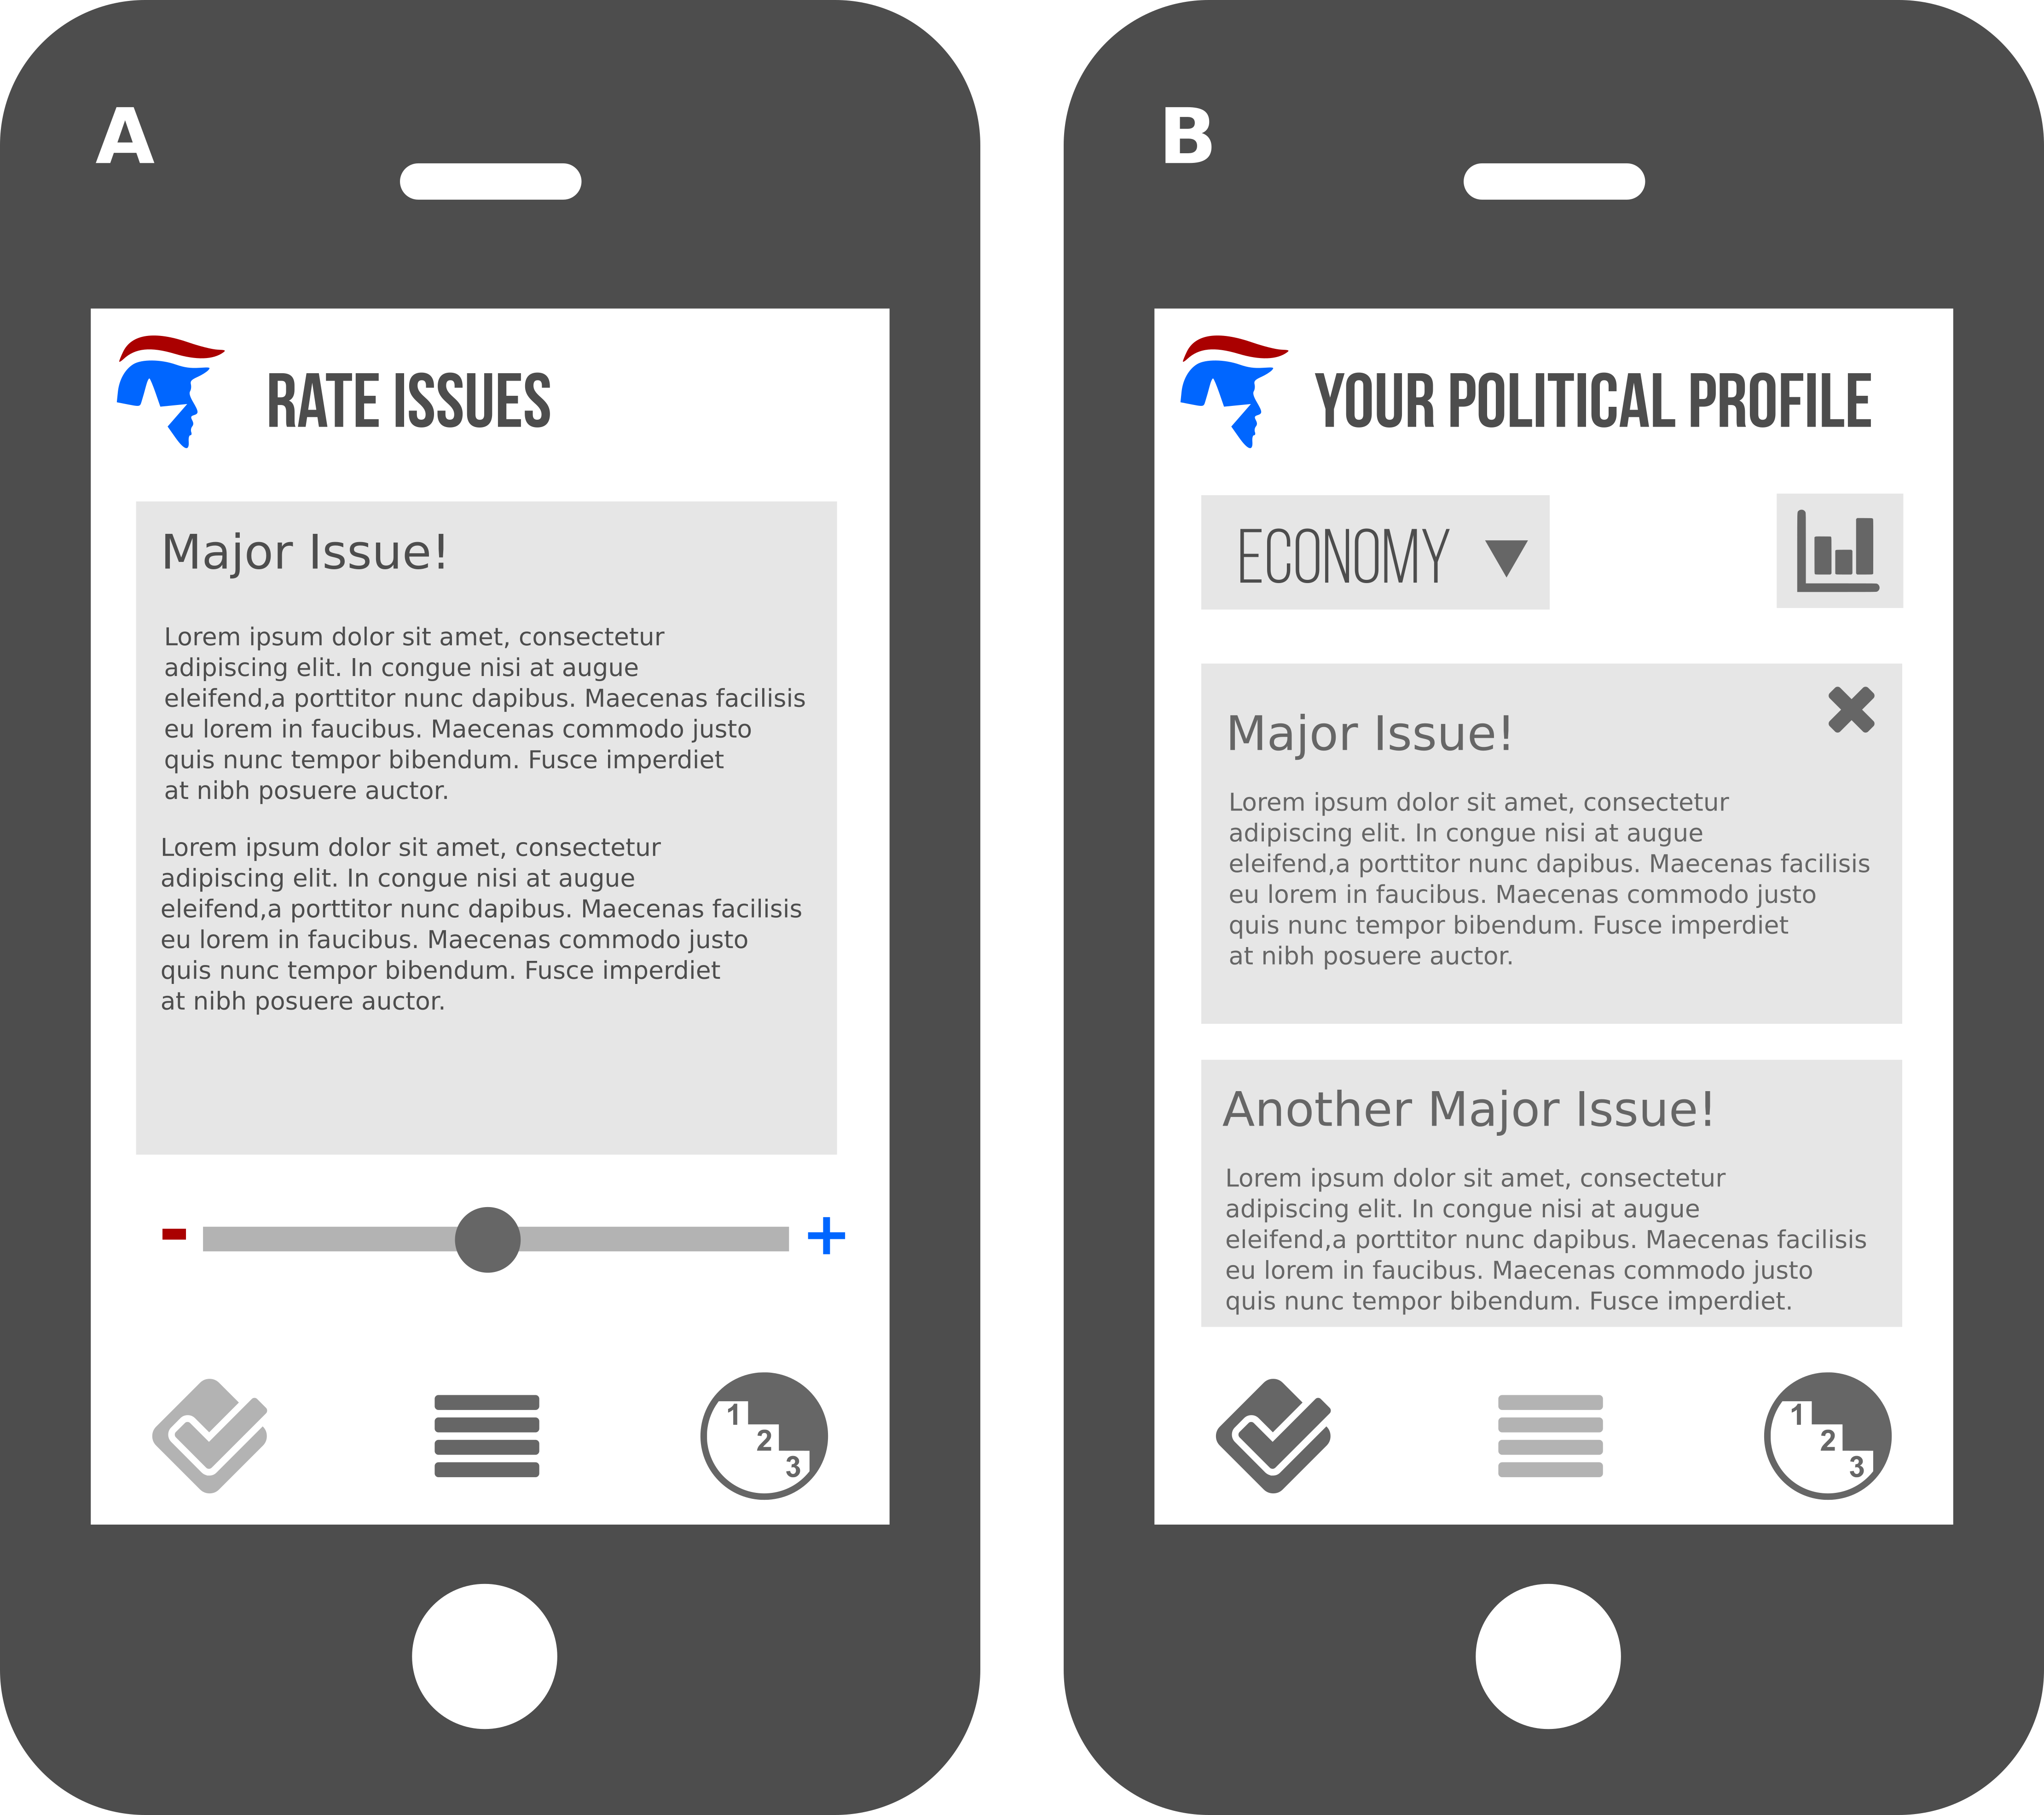
\includegraphics[width = \textwidth]{first.png}
\end{figure}

\begin{description}
    \item[A (left)] Rate Viewpoints. The user is presented with various viewpoints on issues within context of topics such as economics or gun rights. The user then rates each their alignment with the opinion on a continuous scale from negative to positive. The user can then swipe to the next viewpoint.
    \item[B (right)] The user can see the culmination of all their ratings from the Rate Viewpoints flow in a topical feed, along with various visualizations for how they align politically. They can also explore the origin of each viewpoint they have aligned to.
\end{description}

\newpage

\begin{figure}[h]
    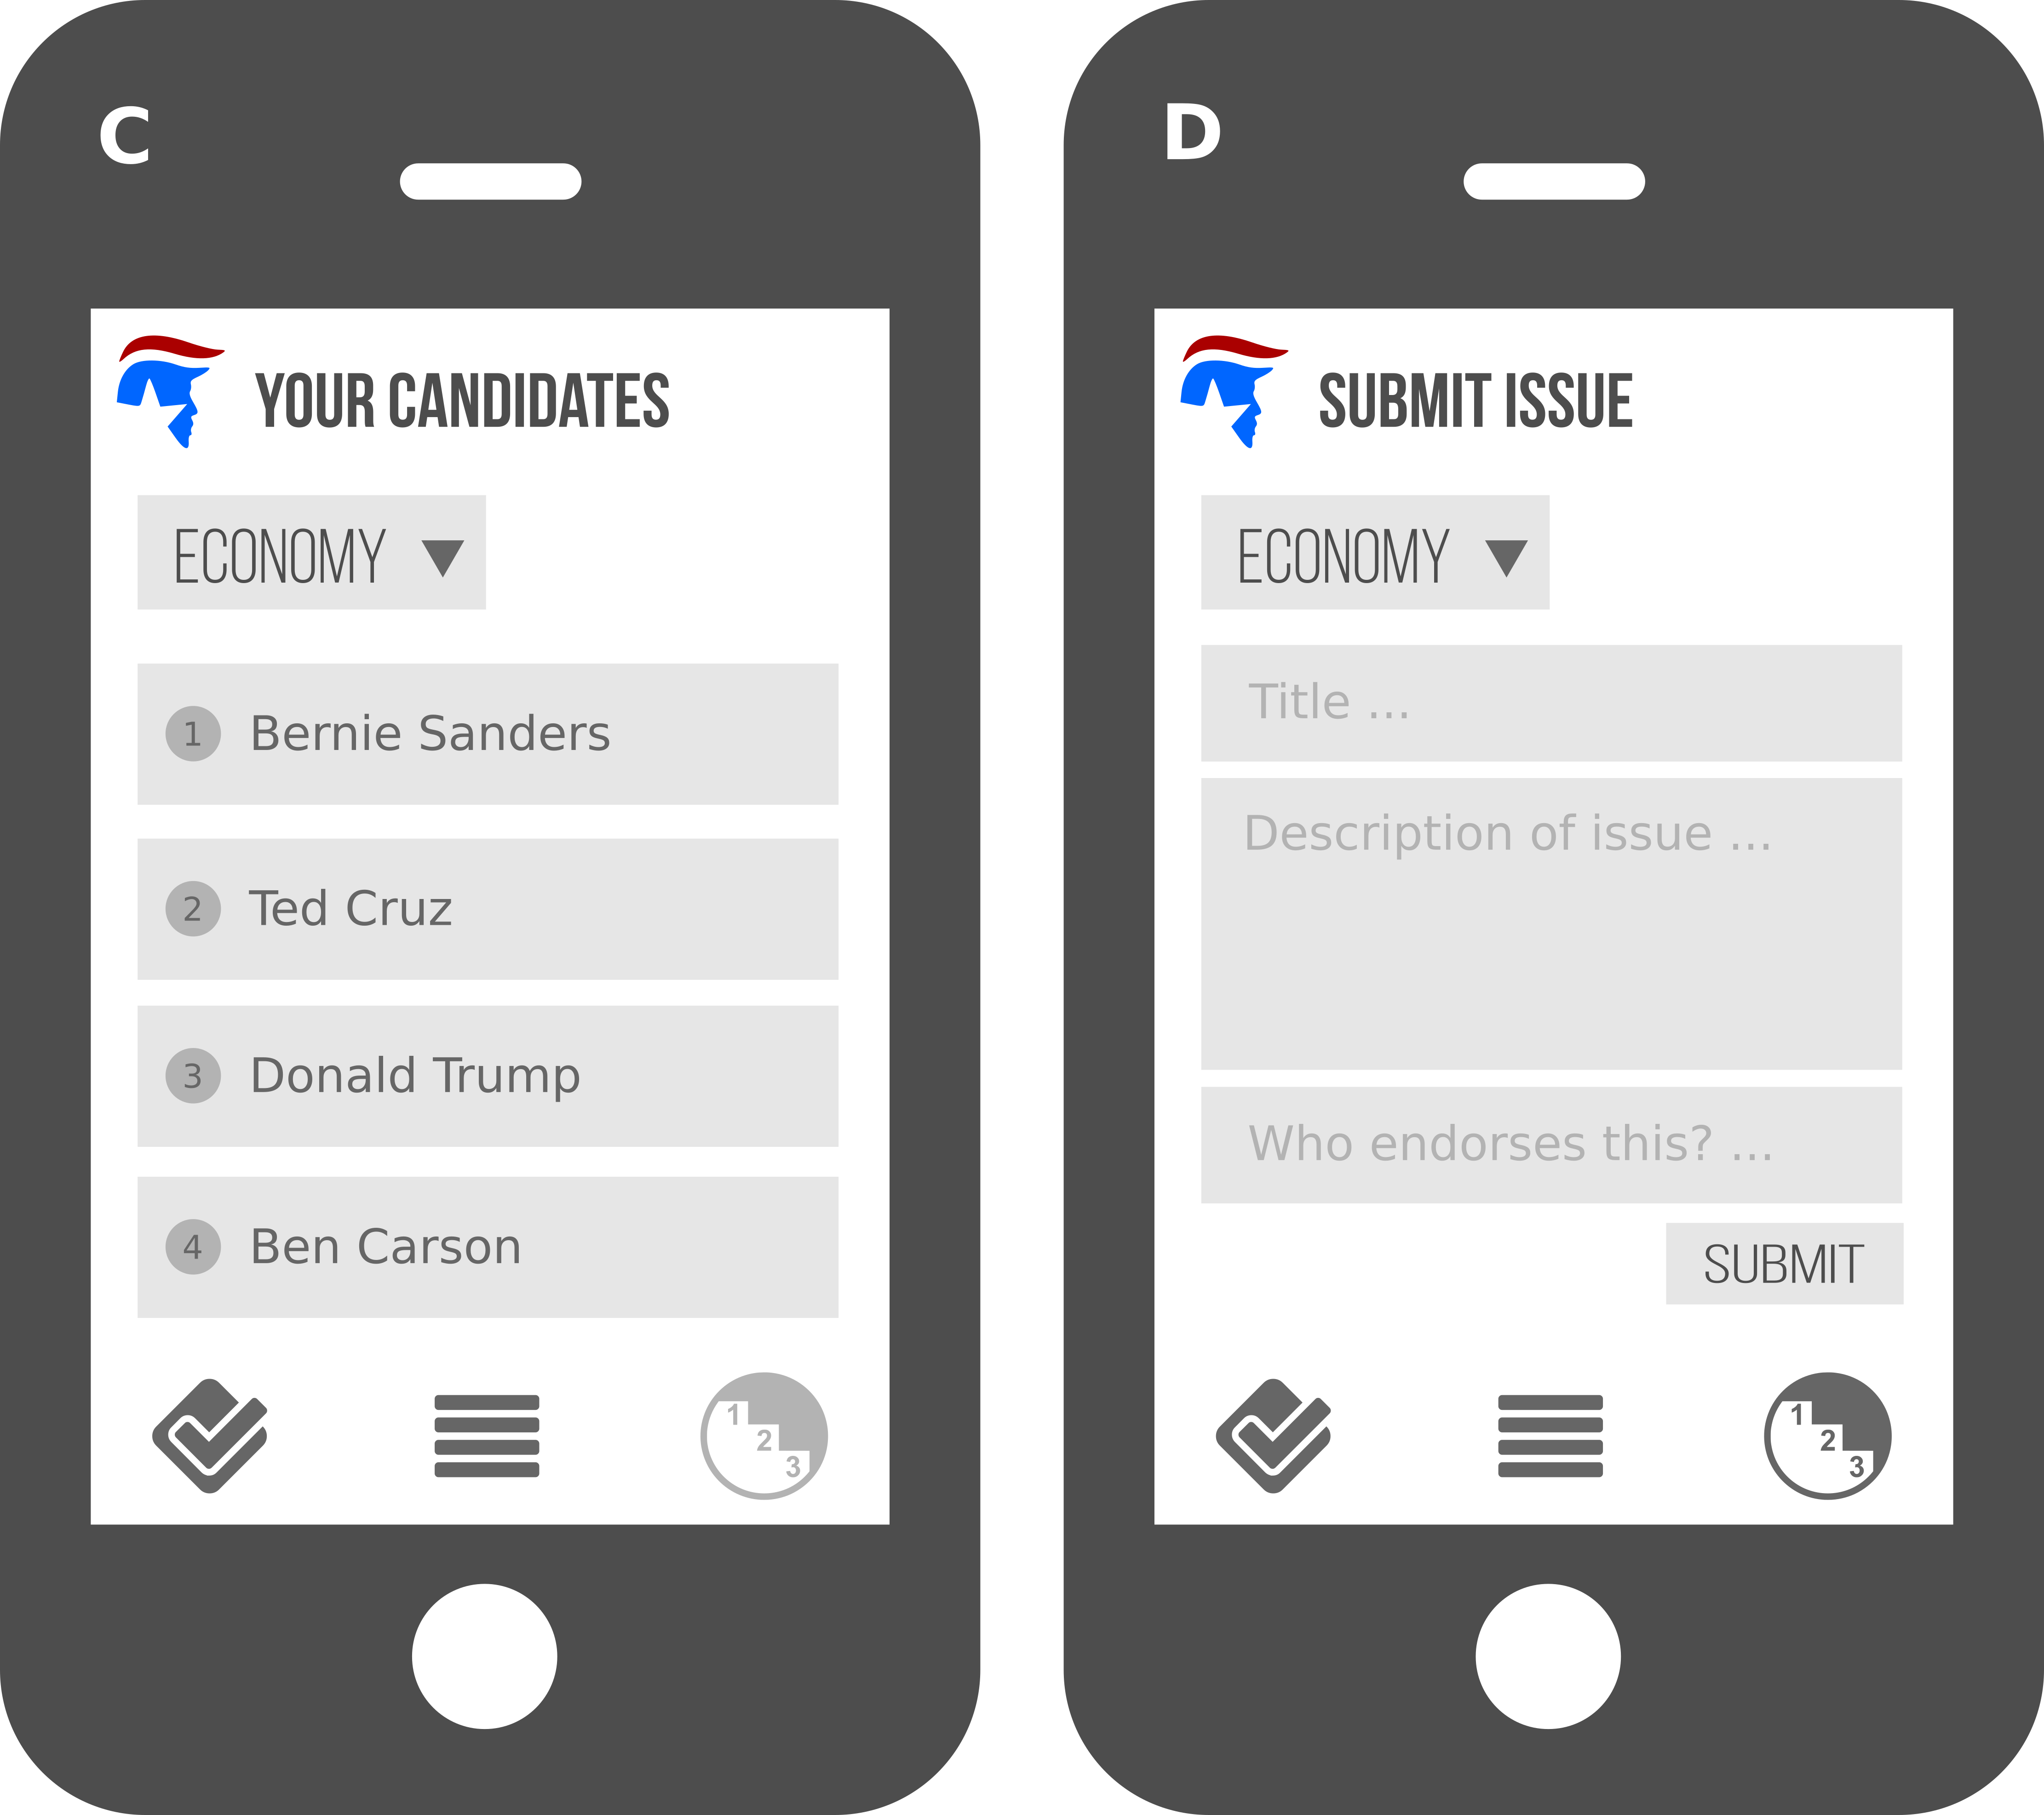
\includegraphics[width = \textwidth]{second.png}
\end{figure}

\begin{description}
    \item[C (left)] Your Candidates. The user can view a list of candidates which most closely align with their political profile on various topics. Candidates are ranked in a scrollable list.
    \item[D (right)] Submit Issue: The user can submit a quote or issue that may be added as a prompt in Rate Viewpoints (A). They submit a title, description of the issue along with the candidate who has previously endorsed the viewpoint. It will be added either through positive user ratings based on previous submissions or by a member of the CYB team manually approving it.
\end{description}

\newpage

\section{Design Changes and Rationale (2/19)}

\subsubsection{Major Features}

We did not make any changes to our major feature requirements and have most of the functionality described about them in this document implemented for the beta release.

\subsubsection{Parse}

Fairly on in the project, it was announced that Facebook was discontinuing support for Parse at the end of 2016. It was decided as a group that we should move away from Parse in order to develop skills that are relevant well after this class ends. As a team, we decided that we should move our implementation over to Firebase, which acts very similar to Parse but will (hopefully) not be discontinued in the near future.

\subsubsection{Timeline}

While our timeline has mostly stayed the same as we have met all of our deadlines that we set as a team, we have fallen slightly behind on the integration of different systems. Specifically, the candidate analysis integration, which should of been completed by February 16th, will not be completed until our Beta release. This will postpone some of the testing that needs to take place in the application by a few days to a week depending on the severity of the delay. This should not have any effect on our beta release or our feature complete release during the following week.

\subsubsection{User Interface}

\begin{tabular}{ccc}
    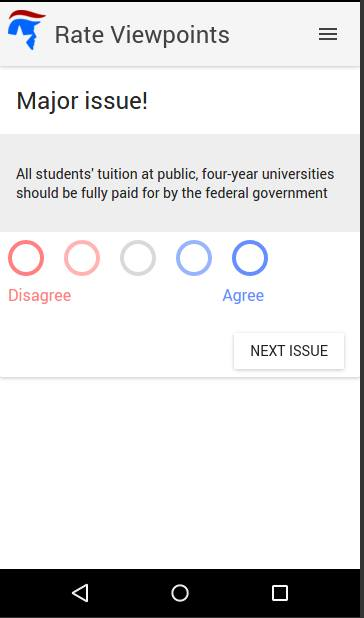
\includegraphics[width = 0.31\textwidth]{1.jpg}
    &
    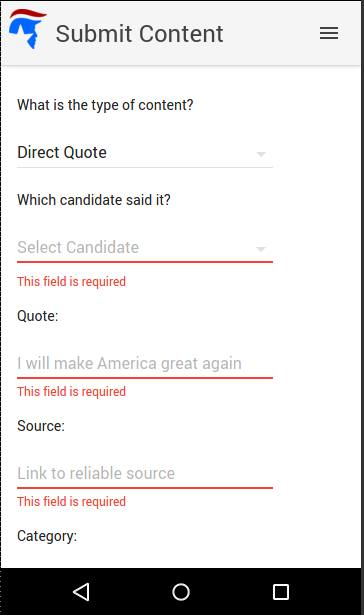
\includegraphics[width = 0.31\textwidth]{2.jpg}
    &
    
\includegraphics[width = 0.31\textwidth]{3.jpg}
\end{tabular}

We made some major changes to the overall design of the UI. Notably, we changed the layout and number of fields in the crowdsourcing view.

\section{Design Changes and Rationale (2/26)}

\subsubsection{iOS Support}

After much effort, we have decided to drop iOS support on this project. In the beginning we chose to use a library called PhoneGap in order to port our web application to both Android and iOS. Unfortunately, we have had to drop support for iOS because some of the main functionality of the app does not work on iOS. Instead of spend engineering hours on debugging and fixing the issue, we have decided to focus our efforts on making the application better / implementing stretch features.

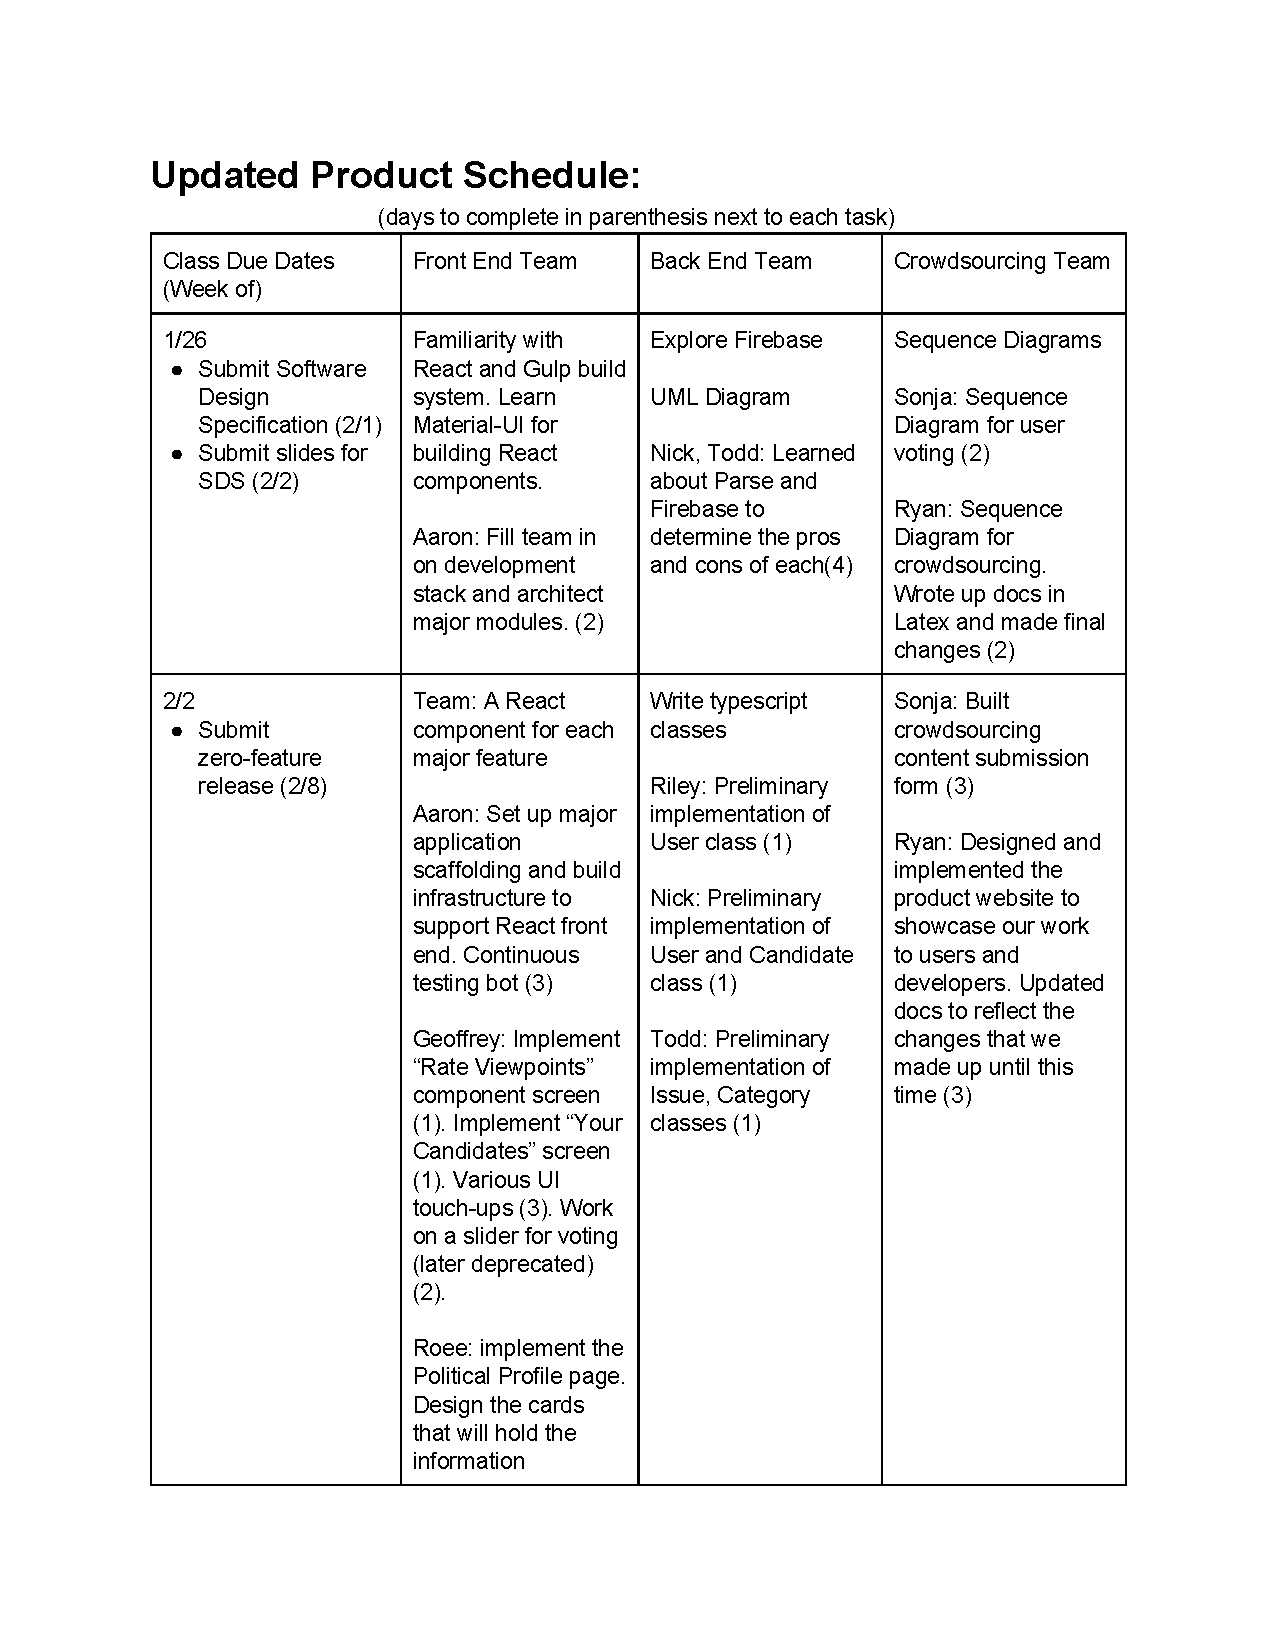
\includepdf[pages=-]{schedule.pdf}

\end{document}
